% Se pre-carga la información del estudiante sólo para poder emplear el macro de
% selección de versión (digital o impresa)
% ===============================================================================
% El estudiante debe llenar sus datos en esta sección para que la plantilla los 
% auto-importe y genere automáticamente las páginas de portada y de firmas 
% autorizadas.
% ===============================================================================
% Datos del estudiante:
% -------------------------------------------------------------------------------
% Nombre completo
\def \nombreestudiante {Gerardo Andres Fuentes Bámaca}
% Carné
\def \uvgcarne {19389}
% Facultad
\def \uvgfacultad {Ingeniería}
% Carrera
\def \uvgcarrera {Ingeniería Mecatrónica}

% Datos del trabajo:
% -------------------------------------------------------------------------------
% Título completo
\def \titulotesis {Implementación de un control de movimiento para dispositivos robóticos móviles utilizando identificación de gestos faciales y orientación de cabeza por medio de visión de computadora}
% Año de entrega
\def \anoentrega {2024}
% Asesor
\def \nombreasesor {PhD. Luis Rivera}

% Datos del tribunal examinador:
% -------------------------------------------------------------------------------
% Nombre del primer examinador
\def \nombreprimerex {MSc. Carlos Esquit}
% Nombre del segundo examinador
\def \nombresegundoex {Ing. Luis Pedro Montenegro}
% Año de aprobación
\def \anoaprobacion {2018}
% Mes de aprobación
\def \mesaprobacion {diciembre }
% Día de aprobación
\def \diaaprobacion {5 }

% Capítulos pre-definidos
% -------------------------------------------------------------------------------
% Comentar las líneas de las secciones que desean omitirse, por defecto se 
% se incluyen todas.
\def \CAPprefacio {Prefacio}
\def \CAPantecedentes {Antecedentes}
\def \CAPalcance {Alcance}
\def \CAPanexos {Anexos}
\def \CAPglosario {Glosario}

% Formato y estilo de la plantilla
% -------------------------------------------------------------------------------
% Modo impresión: Puede des-comentar la siguiente línea para generar un documento pdf sin la portada, para cuando se desee imprimir el documento para encuadernación
\def \printver {Versión del documento para impresión}

% Portada: Puede cambiarse la imagen en la portada al cambiar el nombre del 
% archivo siguiente. NOTA: debe tener la suficiente resolución para cubrir el área
% designada
\def \imagenportada {plantilla/portadacit.jpg}

% Referencias: Puede des-comentar la siguiente línea para utilizar el formato de referencias APA
%\def \usarAPA {Usar formato APA}

% Párrafo: Puede comentar la siguiente línea si desea emplear un formato de 
% párrafo distinto al establecido por defecto
\def \parpordefecto {Formato de párrafo por defecto}

% Capítulos y secciones: Puede des-comentar la siguiente línea para establecer el
% formato de los capítulos y secciones bajo el estándar original de UVG para
% trabajos de graduación. Este incluye: capítulos con numeración romana, secciones
% con letras mayúsculas, sub-secciones con números y sub-sub-secciones con letras
% minúsculas
%\def \capsecuvg {Formato UVG para capítulos y secciones}

\ifdefined\printver
    \documentclass[11pt, letterpaper, twoside, openright]{report}
\else
    \documentclass[11pt, letterpaper]{report}
\fi

% Eliminar la opción de twoside y openright si se desea generar la versión
% digital del documento en lugar de la versión impresa
%\documentclass[11pt, letterpaper, twoside, openright]{report}
\usepackage[spanish, es-nodecimaldot, es-noquoting]{babel}
% cambiar a spanish, mexico si se quiere emplear tabla en lugar de cuadro
\selectlanguage{spanish}
\usepackage[utf8]{inputenc}
\usepackage[T1]{fontenc}

\title{Plantilla para Trabajos de Graduación IE-MT 2019v4}
\author{MSc. Miguel Zea}
\date{\today}

% Información del estudiante en el archivo datos_estudiante.tex
% ===============================================================================
% El estudiante debe llenar sus datos en esta sección para que la plantilla los 
% auto-importe y genere automáticamente las páginas de portada y de firmas 
% autorizadas.
% ===============================================================================
% Datos del estudiante:
% -------------------------------------------------------------------------------
% Nombre completo
\def \nombreestudiante {Gerardo Andres Fuentes Bámaca}
% Carné
\def \uvgcarne {19389}
% Facultad
\def \uvgfacultad {Ingeniería}
% Carrera
\def \uvgcarrera {Ingeniería Mecatrónica}

% Datos del trabajo:
% -------------------------------------------------------------------------------
% Título completo
\def \titulotesis {Implementación de un control de movimiento para dispositivos robóticos móviles utilizando identificación de gestos faciales y orientación de cabeza por medio de visión de computadora}
% Año de entrega
\def \anoentrega {2024}
% Asesor
\def \nombreasesor {PhD. Luis Rivera}

% Datos del tribunal examinador:
% -------------------------------------------------------------------------------
% Nombre del primer examinador
\def \nombreprimerex {MSc. Carlos Esquit}
% Nombre del segundo examinador
\def \nombresegundoex {Ing. Luis Pedro Montenegro}
% Año de aprobación
\def \anoaprobacion {2018}
% Mes de aprobación
\def \mesaprobacion {diciembre }
% Día de aprobación
\def \diaaprobacion {5 }

% Capítulos pre-definidos
% -------------------------------------------------------------------------------
% Comentar las líneas de las secciones que desean omitirse, por defecto se 
% se incluyen todas.
\def \CAPprefacio {Prefacio}
\def \CAPantecedentes {Antecedentes}
\def \CAPalcance {Alcance}
\def \CAPanexos {Anexos}
\def \CAPglosario {Glosario}

% Formato y estilo de la plantilla
% -------------------------------------------------------------------------------
% Modo impresión: Puede des-comentar la siguiente línea para generar un documento pdf sin la portada, para cuando se desee imprimir el documento para encuadernación
\def \printver {Versión del documento para impresión}

% Portada: Puede cambiarse la imagen en la portada al cambiar el nombre del 
% archivo siguiente. NOTA: debe tener la suficiente resolución para cubrir el área
% designada
\def \imagenportada {plantilla/portadacit.jpg}

% Referencias: Puede des-comentar la siguiente línea para utilizar el formato de referencias APA
%\def \usarAPA {Usar formato APA}

% Párrafo: Puede comentar la siguiente línea si desea emplear un formato de 
% párrafo distinto al establecido por defecto
\def \parpordefecto {Formato de párrafo por defecto}

% Capítulos y secciones: Puede des-comentar la siguiente línea para establecer el
% formato de los capítulos y secciones bajo el estándar original de UVG para
% trabajos de graduación. Este incluye: capítulos con numeración romana, secciones
% con letras mayúsculas, sub-secciones con números y sub-sub-secciones con letras
% minúsculas
%\def \capsecuvg {Formato UVG para capítulos y secciones}
% ================================================================================
% En este archivo se colocan opciones adicionales para modificar el formato de la
% plantilla, para emplearse en otros tipos de documentos que no sean trabajos de
% graduación. Si usted está trabajando su tesis, NO modifique este archivo
% ================================================================================
% Capítulos pre-definidos
% --------------------------------------------------------------------------------
% Comentar las líneas de las secciones que desean omitirse, por defecto se 
% se incluyen todas.
\def \CAPportada {Portada}
\def \CAPcaratula {Caratula}
\def \CAPfirmas {Hoja de firmas}
\def \CAPindice {Índice general}
\def \CAPfiguras {Listado de figuras}
\def \CAPcuadros {Listado de cuadros}
\def \CAPresumen {Resumen}
\def \CAPabstract {Resumen}
\def \CAPintroduccion {Introducción}
\def \CAPobjetivos {Objetivos}
\def \CAPjustificacion {Justificación}
\def \CAPmarcoteorico {Marco teórico}
\def \CAPconclusiones {Conclusiones}
\def \CAPrecomendaciones {Recomendaciones}
\def \CAPbibliografia {Bibliografía}

% ==============================================================================
% DEFINICIÓN DE PAQUETES
% ==============================================================================
\usepackage{xcolor}
\usepackage{amsfonts}
\usepackage{amsmath}
\usepackage{amssymb}
\usepackage{amsthm}
\usepackage{amsfonts}
\usepackage{mathtools}
\usepackage{graphicx}
\usepackage{xfrac}
\usepackage{float}
\usepackage{mathtools}
\usepackage[hypertexnames=false]{hyperref}
% \usepackage{bookmark}
\usepackage[font=small]{caption}
\usepackage{subcaption}
%\usepackage{csquotes}
\usepackage{xpatch}
\usepackage{emptypage}
\usepackage{hyphenat}
\usepackage{fancyhdr}
\usepackage[backend=biber, style=ieee]{biblatex}
\ifdefined\usarAPA 
    \usepackage[backend=biber, style=apa]{biblatex}
\fi
\addbibresource{m-bibliografia.bib}

\usepackage[percent]{overpic}

\usepackage{chngcntr}

\ifdefined\CAPglosario
	%\usepackage[toc]{glossaries}
	\usepackage[numberedsection]{glossaries}
	\makeglossaries
    \newglossaryentry{latex}
{
    name=latex,
    description={Es un lenguaje de marcado adecuado especialmente para la creación de documentos científicos}
} 
 
\newglossaryentry{formula}
{
    name=fórmula,
    description={Una expresión matemática} 
}
\fi

% ==============================================================================
% MÁRGENES Y FORMATO GENERALES
% ==============================================================================
\usepackage[top=1in, left=1.5in, right=1in, bottom=1in]{geometry}
%Options: Sonny, Lenny, Glenn, Conny, Rejne, Bjarne, Bjornstrup
\usepackage[Sonny]{fncychap}

% ==============================================================================
% DEFINICIONES DE LA PLANTILLA
% ==============================================================================
\graphicspath{ {figuras/} }
\definecolor{uvg-green}{RGB}{17,71,52}
\newcommand{\defaultparformat}[1]{
	{\setlength{\parskip}{2ex}
     \input{#1}}
}
\ifdefined\capsecuvg
	\renewcommand\thechapter{\Roman{chapter}}
    \renewcommand\thesection{\Alph{section}}
	\renewcommand\thesubsection{\arabic{subsection}}
    \renewcommand\thesubsubsection{\alph{subsubection}}
\fi
\counterwithout{figure}{chapter}
\counterwithout{table}{chapter}
\counterwithout{equation}{chapter}

\newcommand{\blankpage}{
\newpage
\thispagestyle{empty}
\mbox{}
\newpage
}
% ==============================================================================

% Comandos definidos por el usuario en el archivo comandos_usuario.tex
\input{2-paquetes_y_comandos_usuario}

% ==============================================================================
% CUERPO DEL TRABAJO
% ==============================================================================
\pagestyle{headings}
\begin{document}

% ==============================================================================
% PORTADA
% ==============================================================================
\ifdefined\printver
    \let\CAPportada\undefined
\fi 

\ifdefined\CAPportada
    \cleardoublepage\phantomsection
    % \pdfbookmark{Portada}{toc}
	\newgeometry{left=3cm, bottom=0in, top=1in, right=3cm}
	\pagecolor{uvg-green}
	\thispagestyle{empty}

	\color{white}
	\noindent \hrulefill \par
	\vspace{0.1in}
	\noindent \Huge \nohyphens{\titulotesis} \par
	\noindent \hrulefill \par
	\noindent
	\LARGE \nombreestudiante

	\begin{figure}[b!]
    	%\makebox[\textwidth]{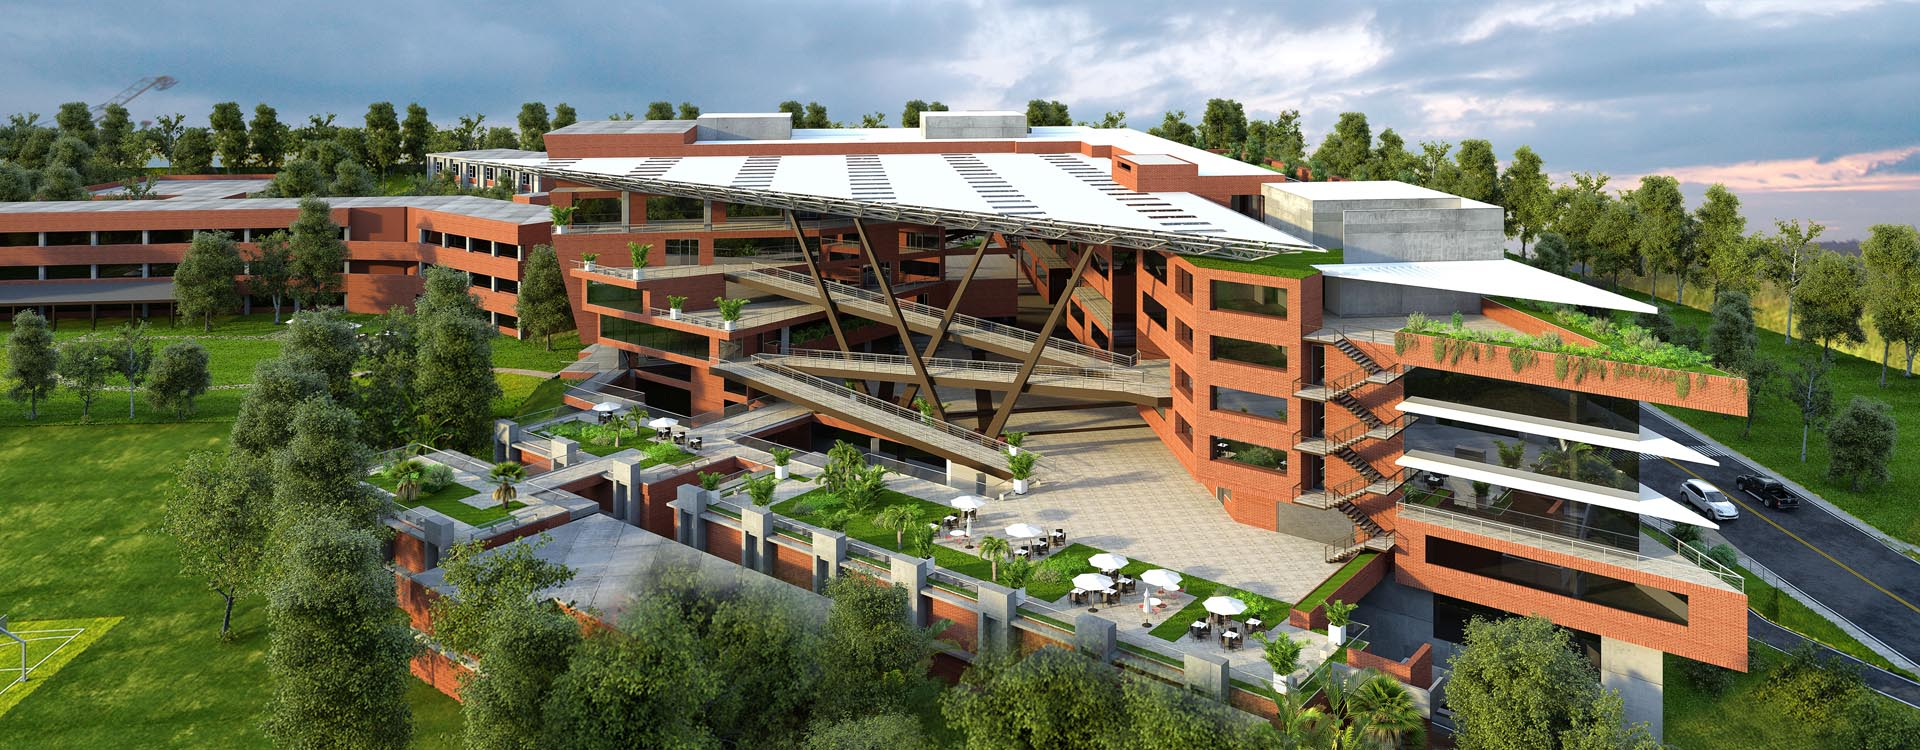
\includegraphics[height=13.25cm]{plantilla/portadacit.jpg}}
    	\makebox[\textwidth]{
    		\begin{overpic}[height=13.25cm]{\imagenportada}
     		\put(63,0){
\includegraphics[height=1.15in]{plantilla/fondologo_grande.png}}  
  			\put(64.5,2){
\includegraphics[height=0.55in]{plantilla/logoUVGblanco.eps}} 
        	\end{overpic}
    	}
    	%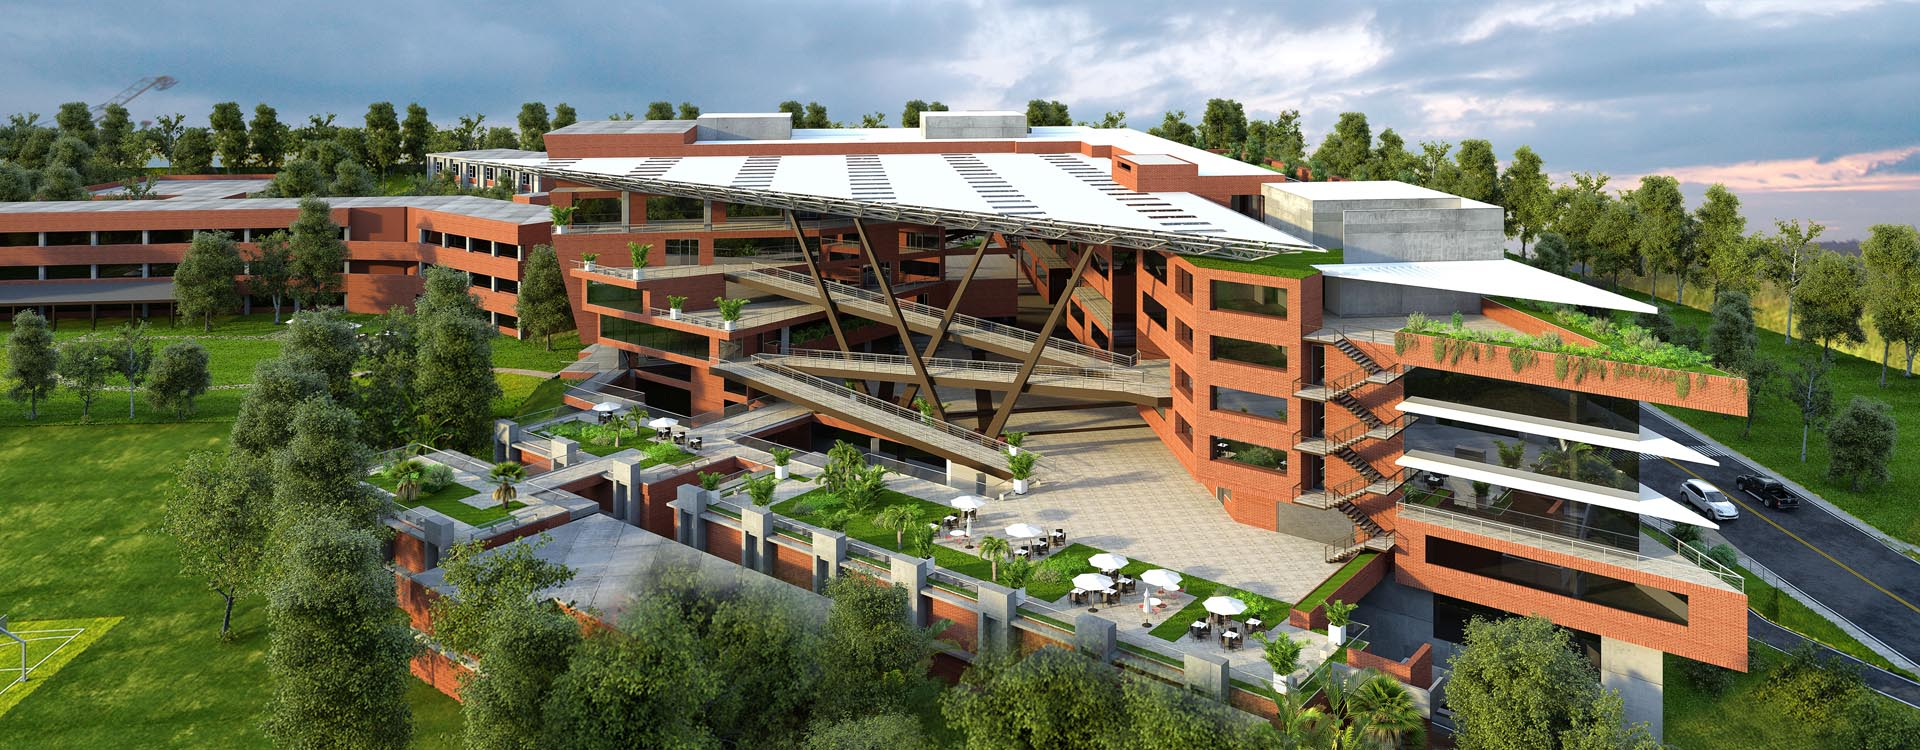
\includegraphics[height=13.25cm]{plantilla/portadacit.jpg}
	\end{figure}
	\restoregeometry
\fi

% ==============================================================================
% PRIMERAS PÁGINAS (Carátulas más hojas de guarda)
% ==============================================================================
\ifdefined\CAPcaratula
	\newpage
    \cleardoublepage\phantomsection
    % \pdfbookmark{Carátula}{toc}
	\pagecolor{white}
	\color{black}
	\setcounter{page}{1}
	\pagenumbering{roman}
	\thispagestyle{empty}
	\begin{center}
		\LARGE UNIVERSIDAD DEL VALLE DE GUATEMALA\\
		\LARGE Facultad de \uvgfacultad \\[0.75cm]
	\end{center}
	\begin{figure}[h]
		\begin{center}
		
\includegraphics[height=5.5 cm]{plantilla/escudoUVGnegro.eps}
		\vspace{0.5in}
		\end{center}
	\end{figure}
	\begin{center}
		\Large \textbf{\nohyphens{\titulotesis}} \\
		%\LARGE \textbf{\titulotesis} \\
		\vfill
		\Large \nohyphens{Trabajo de graduación presentado por \nombreestudiante \ para optar al grado académico de Licenciado en \uvgcarrera} \\
		\vfill
		\large Guatemala, \\
		\vspace{1em}
		\anoentrega
	\end{center}
    
    \ifdefined\printver	
	    \blankpage
	    \blankpage
	    
	    \newpage
	    \cleardoublepage\phantomsection
	    \pagecolor{white}
    	\color{black}
    	\setcounter{page}{1}
    	\pagenumbering{roman}
    	\thispagestyle{empty}
    	\begin{center}
    		\LARGE UNIVERSIDAD DEL VALLE DE GUATEMALA\\
    		\LARGE Facultad de \uvgfacultad \\[0.75cm]
    	\end{center}
    	\begin{figure}[h]
    		\begin{center}
    		
\includegraphics[height=5.5 cm]{plantilla/escudoUVGnegro.eps}
    		\vspace{0.5in}
    		\end{center}
    	\end{figure}
    	\begin{center}
    		\Large \textbf{\nohyphens{\titulotesis}} \\
    		%\LARGE \textbf{\titulotesis} \\
    		\vfill
    		\Large \nohyphens{Trabajo de graduación presentado por \nombreestudiante \ para optar al grado académico de Licenciado en \uvgcarrera} \\
    		\vfill
    		\large Guatemala, \\
    		\vspace{1em}
    		\anoentrega
    	\end{center}
    \fi
\fi

% ==============================================================================
% HOJA DE FIRMAS
% ==============================================================================
\ifdefined\CAPfirmas
	\newpage
	\cleardoublepage\phantomsection
	\thispagestyle{empty}
	\vspace*{0.5in}
	\large Vo.Bo.:\\[1cm]
	\begin{center}
		(f) \rule[1pt]{4 in}{1pt}\\
		\nombreasesor
	\end{center}
	\vspace{1in}

	Tribunal Examinador:\\[1cm]
	\begin{center}
		(f) \rule[1pt]{4 in}{1pt}\\
		\nombreasesor \\[1in]
		(f) \rule[1pt]{4 in}{1pt}\\
		\nombreprimerex \\[1in]
		(f) \rule[1pt]{4 in}{1pt}\\
		\nombresegundoex
	\end{center}
	\vspace{1in}

%	Fecha de aprobación: Guatemala, \rule[1pt]{0.5 in}{1pt} de \rule[1pt]{1 in}{1pt} de \anoaprobacion.
    Fecha de aprobación: Guatemala, \diaaprobacion de \mesaprobacion de \anoaprobacion.
	\normalsize
\fi

% Comentar para formato estilo libro en la numeración de páginas (NO 
% compatible con la guía UVG 2019)
\pagestyle{plain}
% ==============================================================================
% CONTENIDO DEL TRABAJO
% ==============================================================================
% PREFACIO
% ------------------------------------------------------------------------------
\ifdefined\CAPprefacio
	\newpage
	\cleardoublepage\phantomsection
    \chapter*{Prefacio}
    \ifdefined\parpordefecto
    	\defaultparformat{a-prefacio}
    \else
    	Lorem ipsum dolor sit amet, consectetur adipiscing elit. Cras vitae eleifend ipsum, ut mattis nunc. Pellentesque ac hendrerit lacus. Cras sollicitudin eget sem nec luctus. Vivamus aliquet lorem id elit venenatis pellentesque. Nam id orci iaculis, rutrum ipsum vel, porttitor magna. Etiam molestie vel elit sed suscipit. Proin dui risus, scelerisque porttitor cursus ac, tempor eget turpis. Aliquam ultricies congue ligula ac ornare. Duis id purus eu ex pharetra feugiat. Vivamus ac orci arcu. Nulla id diam quis erat rhoncus hendrerit. Class aptent taciti sociosqu ad litora torquent per conubia nostra, per inceptos himenaeos. Sed vulputate, metus vel efficitur fringilla, orci ex ultricies augue, sit amet rhoncus ex purus ut massa. Nam pharetra ipsum consequat est blandit, sed commodo nunc scelerisque. Maecenas ut suscipit libero. Sed vel euismod tellus.

Proin elit tellus, finibus et metus et, vestibulum ullamcorper est. Nulla viverra nisl id libero sodales, a porttitor est congue. Maecenas semper, felis ut rhoncus cursus, leo magna convallis ligula, at vehicula neque quam at ipsum. Integer commodo mattis eros sit amet tristique. Cras eu maximus arcu. Morbi condimentum dignissim enim non hendrerit. Sed molestie erat sit amet porttitor sagittis. Maecenas porttitor tincidunt erat, ac lacinia lacus sodales faucibus. Integer nec laoreet massa. Proin a arcu lorem. Donec at tincidunt arcu, et sodales neque. Morbi rhoncus, ligula porta lobortis faucibus, magna diam aliquet felis, nec ultrices metus turpis et libero. Integer efficitur erat dolor, quis iaculis metus dignissim eu.
    \fi
    \addcontentsline{toc}{chapter}{Prefacio}
\fi

% ÍNDICE GENERAL
% ------------------------------------------------------------------------------
\ifdefined\CAPindice
	\newpage
    \cleardoublepage\phantomsection
	\renewcommand{\contentsname}{Índice}
    %\phantomsection
    \pdfbookmark{\contentsname}{toc}
    %\pdfbookmark{Índice}{toc}
	\tableofcontents
\fi

% LISTADO DE FIGURAS
% ------------------------------------------------------------------------------
\ifdefined\CAPfiguras
	\newpage
    \cleardoublepage\phantomsection
	\renewcommand{\listfigurename}{Lista de figuras}
	\listoffigures
	\addcontentsline{toc}{chapter}{Lista de figuras}
\fi

% LISTADO DE CUADROS
% ------------------------------------------------------------------------------
\ifdefined\CAPcuadros
	\newpage
    \cleardoublepage\phantomsection
	\renewcommand{\listtablename}{Lista de cuadros}
	\listoftables
	\addcontentsline{toc}{chapter}{Lista de cuadros}
\fi

% RESUMEN
% ------------------------------------------------------------------------------
\ifdefined\CAPresumen
	\newpage
    \cleardoublepage\phantomsection
	\chapter*{Resumen}
	\ifdefined\parpordefecto
		\defaultparformat{b-resumen}
	\else
		En una sociedad donde la tecnología los métodos numéricos y cálculos computacionales superan las habilidades humanas, es necesario aplicar nuestro sentido de la empatía y humanidad para poder generar un verdadero desarrollo humano. Una de las ramas en la que se debe trabajar para lograr este desarrollo, es la inclusividad. Con este tema en mente, se plantea un proyecto que logre unir la visión de computadora y la robótica para generar un prototipo de agente móvil el cual pueda funcionar con base en gestos y movimientos faciales. Para esta tarea será importante lograr desarrollar sistemas efectivos de de software y hardware, así como la comunicación entre ellos. 

Para iniciar, se investigará y analizará la disponibilidad de tecnología, tanto software como hardware para implementar visión de computadora a nivel local. Esto se realizará por medio de cotizaciones y análisis de hojas de datos y manuales disponibles, así como la comparación entre plataformas de software. Luego, con los materiales definidos, se procederá a analizar y ajustar los algoritmos y plataformas a utilizar por separado. Después de verificado su correcto funcionamiento se empezará la etapa de desarrollo de algoritmos, en la que se combinarán y probarán las componentes de software, para ser verificadas únicamente por el sensor que se haya seleccionado previamente. Siguiendo esa línea de trabajo, el siguiente paso será verificar la integración del sistema de visión de computadora con simulaciones de agentes robóticos móviles. Cuando los resultados sean satisfactorios, se procederá a migrar este sistema a un agente móvil físico. 



	\fi
	\addcontentsline{toc}{chapter}{Resumen}
\fi

% ABSTRACT
% ------------------------------------------------------------------------------
\ifdefined\CAPabstract
	\newpage
    \cleardoublepage\phantomsection
	\chapter*{Abstract}
	\ifdefined\parpordefecto
		\defaultparformat{c-abstract}
	\else
		This is an abstract of the study developed under the
	\fi
	\addcontentsline{toc}{chapter}{Abstract}
\fi

% INTRODUCCIÓN
% ------------------------------------------------------------------------------
\ifdefined\CAPintroduccion
	\newpage
	\cleardoublepage
	\pagenumbering{arabic}
	\setcounter{page}{1}
	\chapter{Introducción}
	\ifdefined\parpordefecto
		\defaultparformat{d-introduccion}
	\else
		Lorem ipsum dolor sit amet, consectetur adipiscing elit. Quisque eget consequat risus. Praesent a quam lacinia, consequat eros id, auctor tellus. Phasellus a dapibus arcu, vitae luctus leo. Aliquam erat volutpat. Suspendisse ac velit quam. Nullam risus nibh, lobortis vehicula elit non, pellentesque volutpat odio. Donec feugiat porta sapien gravida interdum. Cras odio nunc, lobortis sed pellentesque imperdiet, facilisis eu quam. Praesent pharetra, orci at tincidunt lacinia, neque nulla ornare lacus, ut malesuada elit risus non mi. Fusce pellentesque vitae sapien sed mollis. Curabitur viverra at nulla vitae porta. In et mauris lorem.

Vestibulum faucibus fringilla justo, eget facilisis elit convallis sit amet. Morbi nisi metus, hendrerit quis pellentesque non, faucibus at leo. Proin consectetur, est vel facilisis facilisis, arcu felis vestibulum quam, et fringilla metus neque at enim. Nunc justo mauris, egestas quis maximus eget, viverra vehicula nunc. Fusce eu nulla elementum, condimentum diam at, aliquam leo. Nullam sed sodales enim, eu imperdiet risus. Aliquam ornare augue leo, fringilla mattis nunc facilisis eget. Nam faucibus, libero a aliquet fermentum, magna arcu ultrices lacus, a placerat tortor turpis ut purus.

Integer eget ligula non metus egestas rutrum sit amet ut tellus. Aliquam vel convallis est, eu sodales leo. Proin consequat nisi at nunc malesuada gravida. Aliquam erat volutpat. Aliquam finibus interdum dignissim. Etiam feugiat hendrerit nisl, hendrerit feugiat ex malesuada in. Cras tempus eget arcu vitae congue. Ut non tristique mauris. Vivamus in mattis ipsum. Cras bibendum, enim bibendum commodo accumsan, ligula nulla porttitor ex, et pharetra eros nisl eget ex. Morbi at semper arcu. Curabitur massa sem, maximus id metus ut, molestie tempus quam. Vivamus dictum nunc vitae elit malesuada convallis. Donec ac semper turpis, non scelerisque justo. In congue risus id vulputate gravida. Nam ut mattis sapien.
	\fi
\fi

% ANTECEDENTES
% ------------------------------------------------------------------------------
\ifdefined\CAPantecedentes
	\newpage
	\chapter{Antecedentes}
	\ifdefined\parpordefecto
    	\defaultparformat{e-antecedentes}
    \else
    	\section*{Control de gestos para su uso en automóviles}

El artículo trata sobre el uso del control de gestos como control para conductores sobre los sistemas integrados en automóviles. Se centra en la detección y reconocimiento de gestos manuales mediante técnicas de recolección y procesamiento de imágenes. En primer lugar se resalta la importancia de tener un contraste entre la mano y el fondo para una detección precisa de gestos. Para lograr esto, los se usó un conjunto de LED que emiten luz infrarroja cercana (NIR) con longitud de onda de 950 nm, la cual no es visible para el ojo humano pero si para una cámara CCD modificada. Esta sensor elimina la información de color pero permite la medición de intensidades. \cite{CVVEHI}

El proceso de recolección de imágenes implica segmentar cada imagen utilizando una única clase o categoría, por medio de umbralización simple. Luego, se rastrean y etiquetan los límites de las regiones conectadas con características iniciales como tamaño, alcance, centroide y momentos de Hu. Estas características ayudan a identificar y distinguir diferentes gestos manuales. Después, en una secuencia de imágenes con duración preestablecida, se emparejan regiones correspondientes (denominadas objetos) entre imágenes consecutivas. Esto se realiza al rastrear los centroides y asumiendo que las regiones pequeñas representan un ruido casi nulo. Por último, se calculan características de movimiento como velocidad y aceleración. Esto permite clasificar de objetos en diferentes clases dinámicas. Para reducir el peso computacional, se aplica un método de preselección basado en puntuación difusa y así eliminar algunos objetos. Entonces se utilizan conjuntos difusos para etiquetar objetos en una clase que indica que no son manos, basándose en el análisis de rangos típicos de características para manos. También incluye una fase de reconocimiento, donde los objetos se comparan con gestos de referencia precargados. En este caso se generan funciones de distribución de probabilidad para cada característica, y se mide la similitud entre el objeto observado y la referencia. Para evitar clasificaciones falsas, se determina un umbral por defecto y, si el objeto muestra poco movimiento, se usa un segundo clasificador basado en correlación de forma. La tasa de procesamiento se configuró en 25 fotogramas por segundo con una resolución de 192 $\times$ 144 píxeles y una procesador Pentium-II de 333 MHz. \cite{CVVEHI}


\section*{Reconocimiento de gestos automático para interacciones inteligentes humano-robot}

El enfoque principal de este artículo es el reconocimiento de gestos de cuerpo completo para la interacción inteligente entre humanos y robots. Se describe un método basado en aprendizaje que puede realizar simultáneamente la detección y el reconocimiento de gestos importantes. El método implica la estimación de la pose del cuerpo humano en 3D, el entrenamiento de Modelos Ocultos de Markov (HMM, por sus siglas en inglés) para modelar la variabilidad de patrones, y la construcción de un modelo para gestos no realizados. El método propuesto se integra en un sistema robótico llamado T-Rot y logra un alto rendimiento en el reconocimiento. La metodología utilizada fue la siguiente: 

\subsection*{Modelo humano en 3D:}
Se construyó una base de datos jerárquica del cuerpo humano utilizando imágenes de silueta e imágenes de profundidad. El modelo incluye múltiples niveles para representar diferentes posturas del cuerpo humano. \cite{Lee_2006}

\subsection*{Extracción de características:}
Basado en información sobre las componentes del cuerpo en 3D se seleccionan trece puntos característicos. También se utilizaron los ángulos desde el eje vertical hasta cada punto característico como una característica. \cite{Lee_2006}

\subsection*{Fase de entrenamiento:}
En esta etapa se entrenan los HMM para modelar la variabilidad de los patrones. En este entrenamiento se utilizó la base de datos \textit{KU Gesture} y se aplica el algoritmo K-means para dividir los datos de entrenamiento en sub-categorías. \cite{Lee_2006}

\subsection*{Fase de reconocimiento:}
En la fase de reconocimiento, se utiliza el algoritmo de Viterbi para encontrar la secuencia de estados más probable para un gesto ingresado al modelo. El gesto se detecta y reconoce en función de los HMMs entrenados. \cite{Lee_2006}

\subsection*{Resultados experimentales:}
El método propuesto se evalúa utilizando la base de datos \textit{KU Gesture} y gestos generados. El resultado general de detección es del 94.8 \%, y el resultado de reconocimiento de gestos aislados es del 97.4\%. \cite{Lee_2006}

\section*{Sistema de reconocimiento de manos y rostro para personas ciegas}

Este artículo presenta un sistema de reconocimiento diseñado para ayudar a personas con discapacidad visual. Se han desarrollado sistemas de reconocimiento de gestos con la mano y facial para realizar diversas tareas. El sistema captura imágenes dinámicas de un flujo de video, procesándolas a través de algoritmos respectivos. Para el reconocimiento de gestos con la mano, el sistema primero detecta la región de la mano en imágenes en tiempo real. Esto quiere decir que se realiza conversión del espacio RGB al espacio de color YCbCr. El sistema establece valores umbral superiores e inferiores para la detección de piel, los cuales pueden ser ajustados dinámicamente por el usuario según el entorno. Luego, por medio del algoritmo \textit{Convex Hull} o de envoltura convexa el sistema extrae características de la región de la mano, como las puntas de los dedos y el ángulo entre los dedos. En esta aplicación se reconocen diferentes gestos que representan números del uno al cinco utilizando este sistema. Para el reconocimiento facial, el sistema utiliza clasificadores de cascada Haar y el reconocedor LBPH (Histogramas de Patrones Binarios Locales). La imagen capturada del rostro se convierte a una imagen en escala de grises. Luego, el sistema entrena la base de datos de imágenes utilizando clasificadores y reconocedores. Durante el reconocimiento, la imagen en tiempo real se compara con las imágenes en la base de datos. Si se encuentra una coincidencia, se muestra el nombre asociado con la imagen. \cite{Sharma_2019}


\section*{Sistema de reconocimiento gestos de cabeza utilizando la cámara de gestos}

La Cámara de gestos es una cámara inteligente diseñada para capturar e interpretar gestos de cabeza, aí como expresiones faciales. Esta enfocado principalmente en individuos con discapacidades o parálisis. El documento explora diferentes áreas, como reconocimiento de gestos, detección facial, rastreo de rostro, y detección de obstáculos. Este sistema cuenta con unidades de captura de imágenes, reconocimiento de gestos y la de concentración despliegue de datos. La unidad de captura de imágenes utiliza un sensor de imagen a color CMOS, montada en una placa electrónica. Luego de capturar la secuencia de imágenes o video, la unidad de reconocimiento de gestos analiza e identifica los gestos y expresiones faciales. Para poder realizar esto, utiliza técnicas como modelado de movimiento, análisis de movimiento, reconocimiento de patrones, y \textit{machine learning} para poder interpretar los gestos. Esta unidad también es capaz de detectar el movimiento de la cabeza par luego determinar su orientación. Una vez que los gestos se reconocieron, la información se transfiere a la unidad de concentración y despliegue. Esta unidad puede ser una computadora personal o bien una de control centralizado. La salida de datos de la cámara inteligente, que incluye una descripción de alto nivel del rostro del usuario en diferentes orientaciones, es enviada a la sección de concentración para un futuro procesamiento. \cite{Bankar2015}


\begin{itemize}
	\item Los retos mas importantes afrontados en el desarrollo de dicho sistema fueron:
	\begin{enumerate}
		\item Imágenes fuera del rango de la cámara, esto fue un problema dado que el sistema debe ser capaz de detectar los gestos de movimiento incluso si la cabeza no es completamente visible por el sensor. \cite{Bankar2015}
		\item La variación de las condiciones de iluminación, el sistema también debe ser capaz de reconocer los gestos de la cabeza con precisión aún si las condiciones de luz cambian, entendiendo que esto puede cambiar el aspecto del rostro del usuario. \cite{Bankar2015}
		\item La variación de las formas de los rostros, los usuarios jamás tendrán rostros exactamente iguales, tanto por forma, tono de piel, bello facial, gafas, entre otros, dicha variación provoca un mayor reto para reconocer gestos de manera adecuada. \cite{Bankar2015}
		\item Fondos desordenados, cuando el dispositivo móvil realice una acción de movimiento, el fondo puede parecer desordenado o en movimiento, lo cual se puede mezclar con el movimiento de los gestos, creando así una dificultad para diferenciar el fondo de los gestos en el algoritmo de reconocimiento del sistema. \cite{Bankar2015}
	\end{enumerate}
\end{itemize}

\section*{Control de una silla de ruedas usando una agrupación de k-medias adaptativas de las poses de la cabeza}


En este artículo se presenta la idea de ayudar a las personas con ciertas discapacidades físicas, por modio de una interfaz que utiliza el sensor Kinect desarrollado por Microsoft. El objetivo es permitir a las personas con discapacidades interactuar con los dispositivos electrónicos. Para lograr esto, se utilizó un algoritmo basado en la Regresión de Bosques Aleatorio y uno de agrupación de k-medias para detectar los cambios en el rango de dirección de los movimiento de cabeza. Y la experimentación se realizó en 5 individuos operando la silla de ruedas en condiciones favorables y no favorables. \cite{LuisA2013}

El sistema propuesto se basa en el método de agrupamiento de k-medias, el cual es un esquema de agrupamiento que utiliza puntos representativos y distancias euclidianas para medir escala de similitud entre vectores y el agrupamiento de puntos representativos. Además los datos obtenidos son posibles gracias al sensor de profundidad utilizado. La arquitectura del sistema propuesto funciona de la siguiente manera: 

\subsection*{Calibración}

Este proceso consta del establecimiento de la configuración inicial para cada usuario, del tal manera que se pueda realizar un proceso personalizado al usuario. Este proceso requiere que el usuario coloque la posición de la cabeza según solicite la interfaz, para configurar las funciones de detenerse, izquierda, derecha, adelante y atrás. Este proceso utiliza el algoritmo RRF. Luego, los datos recopilados se guardan para luego utilizarse en el proceso de adaptación. \cite{LuisA2013} 

\subsection*{Rectificado}
Esta es la etapa final, pero el artículo lo menciona que es importante mencionar en este punto la funcionalidad del proceso. Dado que el sistema se encuentra generando constantemente estimados de los ángulos de pose, es importante realizar un rectificado según la pose y la capacidad de movimiento del usuario. \cite{LuisA2013} 

\subsection*{Adaptación}

Se consideró que, dadas las situaciones de fatiga o degeneración en las enfermedades de los usuarios, podría suceder una descalibración del control de movimiento. Para esto se integraron dos métodos al sistema. El primer método consisten en la implementación de sensores de sonar que se encargan de detectar obstáculos. Al detectarlos, se implementa una corrección en el movimiento. El siguiente método consiste en crear agrupaciones adicionales a las de las funciones principales. Dichas agrupaciones, son las combinaciones de los movimientos básicos. Esto es realizado por medio de el algoritmo de agrupamiento de k-medias, y ayuda a no realizar cambios de movimiento abruptos. \cite{LuisA2013} 



    \fi  
\fi

% JUSTIFICACIÓN
% ------------------------------------------------------------------------------
\ifdefined\CAPjustificacion
	\newpage
	\chapter{Justificación}
	\ifdefined\parpordefecto
		\defaultparformat{f-justificacion}
	\else
		Para llegar a ser una sociedad más inclusiva es necesario poder desarrollar tecnología que afronte diferentes situaciones, en este caso las personas con algún tipo de discapacidad. Existe una gran variedad de extremidades inhabilitadas en el espectro de las discapacidades. En muchos casos bastaría con un sistema de reconocimiento de gestos de manos para personas con parálisis de la cintura para abajo. Sin embargo, también hay que tomar en cuenta a las personas con discapacidades en las extremidades superiores, es ahí donde entra el reconocimiento de gestos de la cabeza. El desarrollo de un sistema de visión de computadora capaz de reconocer gestos faciales/de cabeza, que sea capaz de enviar comandos a un robot móvil es el primer paso para desarrollar una tecnología de apoyo. El control de un robot móvil por medio de este algoritmo, dará paso a una futura migración de comandos a plataformas móviles como sillas de ruedas, o bien vehículos eléctricos. Esta alternativa también busca utilizar sensores mucho más comunes en el mercado, como lo son los sensores de imágenes a comparación de sensores de profundidad o bien de señales bioeléctricas. Los sensores de imágenes, además tienen el valor agregado de brindar una mayor libertad de movimiento a los usuarios, ya que no son intrusivos, por lo que el gesto realizado tiende a una mayor naturalidad. Esto sucede dado que al utilizar aquellos que funcionan con EEG o EMG, requieren dispositivos de extensión al cuerpo humano, como son gorras, guantes o electrodos adheridos al cuerpo del sujeto de prueba. Por otro lado, también se espera que la sección de corrección por integración de sensores, permita una mayor seguridad al usuario. \cite{Wang_Jang_2018}, \cite{Bankar2015}






	\fi
\fi

% OBJETIVOS
% ------------------------------------------------------------------------------
\ifdefined\CAPobjetivos
	\newpage
	\chapter{Objetivos}
	\ifdefined\parpordefecto
		\defaultparformat{g-objetivos}
	\else
		
\section*{Objetivo general}
Desarrollar un sistema de visión por computadora para reconocimiento de gestos y orientación de la cabeza para el control de un agente robótico móvil.

\section*{Objetivos específicos}
\begin{itemize}
	\item Investigar y seleccionar el hardware y software disponible para la aplicación de visión por computadora.
	
	\item Implementar un algoritmo de visión por computadora para reconocimiento de gestos y movimiento de la cabeza.
	
	\item Implementar un algoritmo de traducción de los gestos y movimientos de la cabeza a comandos de control para el agente robótico.
	
	\item Validar el correcto funcionamiento del sistema de reconocimiento y control por medio de simulaciones computarizadas. 
	
	\item Validar el correcto funcionamiento del sistema de reconocimiento y control por medio de plataformas robóticas móviles. 
	
\end{itemize}
	\fi
\fi

% ALCANCE
% ------------------------------------------------------------------------------
\ifdefined\CAPalcance
	\newpage
	\chapter{Alcance}
	\ifdefined\parpordefecto
    	\defaultparformat{h-alcance}
    \else
    	Podemos usar \Gls{latex} para escribir de forma ordenada una \gls{formula} matemática. 
    \fi 
\fi

% MARCO TEÓRICO
% ------------------------------------------------------------------------------
\ifdefined\CAPmarcoteorico
	\newpage
	\chapter{Marco teórico}
	\ifdefined\parpordefecto
		\defaultparformat{i-marco_teorico}
	\else
		\section*{Visión por computadora}

Como humanos percibimos el mundo tridimensional con bastante facilidad, esto es ejemplificado al momento de hacer la diferenciación entre los detalles de macetas o bien contar personas o interpretar sus emociones en un retrato grupal. Replicar este proceso es una tarea que tanto los psicólogos e investigadores de visión por computadora han intentado por años. Mientras que las ilusiones ópticas nos ofrecen algunos indicios, el entendimiento por completo aún es incierto. En el mundo de la visión por computadora, se han hecho avances en técnicas matemáticas para reconstruir formas e imágenes tridimensionales, el seguimiento de objetos, e incluso el reconocimiento de personas en fotografías. Sin embargo, alcanzar una interpretación de imágenes comparable a la de niños pequeños aún es un reto. La visión posee dificultades dado que es un problema de ingeniería inversa, el cual requiere modelos basados en física y estadística para navegar en la ambigüedad. Actualmente, la visión por computadora tienen sus cimientos en dichos modelos de física y gráficas de computadora, abordando problemas sobre cómo se mueven los objetos, el reflejo de la luz e interacción con el ambiente. Hoy, la visión de computadora es subestimada por personas externas debido a una malentendido con respecto al funcionamiento, esta es una creencia refutada, esta afirmaba que la percepción era más simple que el pensamiento cognitivo. En la actualidad,  existen muchas aplicaciones de visión por computadora, las cuales tienen diferentes retos respecto de su complejidad en matemáticas, o de la naturaleza misma del problema. En visión de computadora, es sumamente importante aplicar métodos o técnicas que se acoplen al problema o reto en vez de producir métodos genéricos. De esta manera se genera un pensamiento ingenieril para la resolución de problemas, dado que muchas veces se requiere modelos de la física del caso y así como la estadística para modelar escenarios y el ruido que se pueda obtener un escenario más fiel a la realidad. \cite{Szeliski_2023}

El campo de la visión por computadora es una ramificación de la inteligencia artificial, la cual tiene el propósito de utilizar computadoras y sistemas para poder obtener información importante desde imágenes, videos u otros datos visuales, para luego poder realizar acciones. Este campo es un sistema que se forma con componentes de \textit{hardware}, los cuales pueden ser cámaras, iluminación, lentes, sensores de imágenes, etc. Además, también deben poseer una sección de \textit{software}, que se refiere a los algoritmos para procesar y analizar imágenes, videos, etc. También, es necesario tomar en cuenta la comunicación entre el \textit{hardware} y \textit{software}, dado que esto es lo que permite el funcionamiento del sistema, para esto existen diferentes protocolos. \cite{IBM}

\subsection*{Procedimientos}
\subsubsection*{Clasificación de imágenes:}

Es el proceso de categorizar o etiquetar imágenes en diferentes clases o cateogrías predefinidas. Esto incluye el entrenamiento de un modelo de \textit{Machine Learning} para reconocer y diferenciar entre los diferentes objetos, escenarios, o patrones de imágenes. El objetivo es desarrollar un modelo que pueda clasificar de manera eficaz imágenes nuevas o no antes vistas, basado en los patrones y características que se han aprendido previamente. La clasificación de imágenes tiene muchos campos, como detección de objetos, detección de rostros, imágenes médicas, y vehículos autónomos. El proceso para realizar la clasificación de imágenes sigue de la siguiente manera: 

\paragraph*{Recolección de datos:}
En esta etapa se debe recolectar un grupo grande de imágenes las cuales estén previamente etiquetadas en clases o categorías específicas.\cite{Krizhevsky}
\paragraph*{Procesamiento de datos}
Esta parte se encarga de limpiar y realizar un proceso previo a las imágenes de tal manera que aseguren que tienen el formato adecuado para ingresar al modelo. Esta etapa incluye, reajuste de tamaño o proceso de normalizado. \cite{Krizhevsky}
\paragraph*{Extracción de características:}
En este caso se extraen características únicas de las imágenes que ayuden a distinguir entre clases, esto se puede hacer con diferentes técnicas como redes neuronales convolucionales o con otro métodos menos automáticos. \cite{Krizhevsky}
\paragraph*{Entrenamiento del modelo:}
Para poder evaluar el modelo, se necesita un grupo de datos separado, para verificar el rendimiento. Las métricas de evaluación normalmente son: exactitud, precisión, \textit{recall}, y la calificación F1. \cite{Krizhevsky}
\paragraph*{Optimización del modelo:}
Ajustar el modelo es posible utilizando los hiperparámetros, como la optimización del proceso de entrenamiento, o usando técnicas como la regularización.\cite{Krizhevsky}
\paragraph*{Predicción:}
Ya que el modelo está entrenado y optimizado, se puede usar para clasificar nuevos datos, o datos no antes vistos, y este devuelve la categoría o clase en la que fue clasificado el dato o imagen. \cite{Krizhevsky}

\subsubsection*{Detección de objetos:}
La detección de objetos es una técnica de visión por computadora para localizar instancias de objetos en imágenes o videos. Los algoritmos de detección de objetos suelen aprovechar el aprendizaje automático o el aprendizaje profundo para producir resultados significativos. La detección de objetos es una tecnología clave detrás de los sistemas avanzados de asistencia al conductor (ADAS) que permiten a los automóviles detectar carriles de conducción o realizar la detección de peatones. La detección de objetos también es útil en aplicaciones como sistemas de vigilancia de video o sistemas de recuperación de imágenes. \cite{MATHOD}

\subsubsection*{Estimación de pose:}
Es el proceso de determinar la posición y orientación de un objeto en un sistema de coordenadas. Se usa comúnmente en visión de computadora y aplicaciones robóticas. En el contexto de estimación de pose de cámaras, el objetivo es determinar la posición y orientación de una cámara relativa al escenario tridimensional. Esto se realiza normalmente, por medio del emparejamiento de los puntos en imágenes 2D con sus puntos correspondientes en el espacio 3D. Este proceso incluye resolver el problema de la Perspectiva en punto o \textit{Perspective-n-Point}, el cual implica encontrar la pose de una cámara dado un grupo de puntos correspondientes entre el plano 2D y el espacio 3D. Para realizar la estimación de pose existen muchos métodos, incluyendo iterativos y no iterativos. Los métodos iterativos realizan una refinación del estado inicial por medio de un proceso de estimación. Por otro lado, los métodos no iterativos calculan la pose una única vez, sin iteraciones. Un método popular no iterativo es el algoritmo EPnP (\textit{Efficiente Perspective-n-Point}), que está basado en la resolución de un grupo de ecuaciones lineales. Esta utiliza una suma ponderada de puntos de control virtuales para representar puntos en tres dimensiones y reducir el problema a la estimación de las coordenadas de dichos puntos. Este método es computacionalmente eficiente y devuelve resultados precisos. \cite{3dpose1}

\subsubsection*{Rastreo de objetos:}
En visión de computadora el rastreo de datos involucra la aplicación de algoritmos para detectar y seguir el movimiento de objetos específicos dentro de un video o a lo largo de cuadros. Este proceso es esencial para varias aplicaciones, desde el rastreo de robots en bodegas hasta el rastreo en sistemas de drones. El rastreo tiene sus pilares en la detección de objetos, sin embargo el objeto puede tener distintas apariencias dependiendo de los escenarios y los ángulos. El algoritmo de rastreo predice la posición de un objeto en cuadros de imagen consecutivos, al mismo tiempo que identifica y sigue más de un objeto en una imagen o video. El proceso de rastreo de objetos inicia con la definición del objeto de interés, esto se hace encerrando al objeto en un recuadro, en el primer cuadro del video. El algoritmo de rastreo, luego estima o predice la posición en los cuadros restantes mientras vuelve a encerrar al objeto en ese recuadro de manera simultánea. El algoritmo para rastreo de objetos puede clasificarse basado en el número de objetos que rastrean, incluyendo el rastreo de un único objeto, el cual implica rastrear un objetivo a la vez, y el rastreo múltiple de objetos. Los algoritmos de rastreo tienen muchos retos como ambientes complejos, y la aplicación de diferentes técnicas, como el aprendizaje profundo. El rastro de objetos es una tarea importante en la visión de computadora por sus aplicaciones en, monitoreo de tráfico, robótica, imágenes médicas, etc. \cite{Walia_2022} \cite{Acharya_2023} \cite{Barla_2021} \cite{Klingler_2023}


\subsubsection*{Reconocimiento de gestos:}

La interacción entre computadoras y humanos existe de diferentes maneras, pero la interacción por medio de gestos tiene un pesos importante dado que, le permite a los humanos una mayor naturalidad al momento de comunicarse. Hoy, existen diferentes métodos para reconocimiento de gestos, los cuales requieren dispositivos que sirven como extensión al cuerpo humano. Sin embargo, estos limitan la naturalidad con que un sujeto de prueba puede interactuar con su ambiente. La alternativa que se propone, desde hace más de veinte años, es la visión de computadora, dado que para capturar los gestos de la persona únicamente se requiere una cámara . Actualmente, el reconocimiento de gestos por visión de computadora está basado en su mayor parte en el \textit{Hidden Markov Model (HMM)}, los algoritmos de redes neuronales y el algoritmo de redondeo del tiempo dinámico. Los pasos para realizar dicho reconocimiento, son: recopilación de imágenes, segmentación de manos, reconocimiento de gestos y clasificación. \cite{Wang_Jang_2018}


La recolección de imágenes se divide en dos partes fundamentales, RGB y de profundidad. Comúnmente, se utiliza únicamente cámaras para detectar el RGB, sin embargo, para la profundidad es necesario utilizar otro tipo de sensores, los cuales puedan devolver información de profundidad. Además, para poder analizar correctamente los gestos es necesario también dividirlos entre estáticos y dinámicos. Dicha división se refiere a la distinción entre fotos o videos respectivamente. Lastimosamente, el proceso de recolección de imágenes se ve afectado por problemas de dirección e intensidad de luz, por lo que los algoritmos realizados deben apuntar a ser invariantes respecto iluminación. \cite{Wang_Jang_2018}



\subsection*{Hardware}
\subsubsection*{Cámaras o sensores de imágenes:}

Los sensores de las cámaras digitales son dispositivos electrónicos que contienen millones de píxeles fotosensibles, estos registran la cantidad de luz que reciben. Al presionar el botón para tomar la fotografía, se descubren los píxeles para recoger los fotones y almacenarlos como una carga eléctrica. Cuando termina la exposición a la luz, la cámara cierra cada uno de estos píxeles y luego revisa cuántos fotones cayeron, midiendo así, la intensidad de la señal eléctrica. Estos datos se guardan como valores digitales, y su precisión es determinada por la profundidad de bits. Luego, los datos se procesan y convierten en una imagen que se guarda en una tarjeta de memoria o en la cámara por sí misma. En la actualidad, estos sensores se utilizan en cámaras digitales, módulos de cámara, teléfonos con cámara, equipos de imágenes médicas, dispositivos de visión nocturna, etc. En productos de consumo diario normalmente utilizan sensores \textit{Semiconductores complementarios de óxido metálido} o CMOS, por sus siglas en inglés, los cuales son en su mayoría más baratos y su consumo de energía es bajo en dispositivos con batería. Por otro lado, los sensores \textit{Dispositivos de carga acoplada} o CCD, por sus siglas en inglés, se utilizan en cámaras de video de alta calidad. Ambos tipos de sensores cumplen la misma tarea de capturar luz y convertirla en señales eléctricas. Los sensores de imagen también pueden tener diferentes tamaños y resoluciones, lo cual afecta la calidad de la imagen. Los sensores más grandes tienen una mayor capacidad para capturar luz y, por ende, pueden producir imágenes de mayor calidad y con menor ruido. Además, los sensores de imagen también pueden tener diferentes formatos, como el \textit{Full-frame}, el formato APS-C y el formato \textit{Micro Four Thirds}, que afectan el ángulo de visión y la profundidad de campo. \cite{RadhaKrishna}

\subsubsection*{Sensor LiDAR:}


LiDAR, o \textit{Light Detection and Ranging}, es una tecnología de teledetección, y funciona al emitir pulsaciones láser y luego midiendo el tiempo que tarda la luz en regresar después de golpear un objeto o la superficie terrestre. Al medir el tiempo de los pulsos con precisión, los sistemas LiDAR pueden calcular la distancia al objeto o superficie. Este proceso se repite varias veces para crear un mapa tridimensional detallado. Los datos resultantes suelen representarse como un sistema de coordenadas tridimensional. En los vehículos autónomos, LiDAR es un componente importante que les permite percibir y navegar su entorno con alta precisión y exactitud. En robótica, se utiliza para la localización y mapeo simultáneos, lo que permite a los robots crear mapas de su entorno y navegar dentro de él. También, se usa para crear mapas altamente detallados del terreno, vegetación y cobertura terrestre, lo cual ayuda a la gestión ambiental y de agricultura. En la planificación urbana, los datos se utilizan para crear modelos tridimensionales detallados de ciudades, par evaluar infraestructuras. Las ventajas de este sistema incluyen: datos tridimensionales altamente precisos y detallados, que lo hace valioso para diversas aplicaciones que requieren información espacial. También, puede utilizarse en diversos entornos y para muchas aplicaciones, como la gestión ambiental y desarrollo de infraestructuras mencionadas anteriormente. Además tiene la capacidad de capturar rápidamente grandes cantidades de datos, lo que permite un eficiente mapeo y topografía de áreas extensas. Por otro lado, sus mayores desventajas radican en el alto costo y en la baja compatibilidad de los datos recopilados. \cite{XinWang}

\subsubsection*{Sensor RADAR:}
Estos dispositivos convierten las señales de eco de microondas en señales eléctricas, utilizando tecnología inalámbrica para detectar el movimiento por medio de la posición, forma, tipo de movimiento y trayectoria de un objeto. A diferencia de otros sensores, no se ven afectados por el espectro de luz, y tienen la capacidad de detección aunque existan obstáculos de por medio. Una de sus principales ventajas es su capacidad para detectar el movimiento al calcular la velocidad y dirección de un objeto a través del efecto Doppler, así como observar el movimiento del objetivo desde diferentes perspectivas usando sensores multicanal. Los sensores de radar se utilizan cada vez más en dispositivos portátiles, edificios inteligentes y vehículos autónomos, y su importancia histórica es evidente en aplicaciones como la predicción del clima y el seguimiento de la temperatura.  \cite{Atwell_2021}

Estos sensores funcionan detectando la radiación electromagnética transmitida y reflejada. Envían pulsos electromagnéticos cronometrados y analizan la diferencia entre las señales enviadas y recibidas para detectar el movimiento, la presencia, la distancia, la velocidad y la localización de objetos. Estos sensores se utilizan en una gran variedad de campos donde se requiere una acción automática al detectar un objeto en movimiento, como controlar luces, sistemas de calefacción y refrigeración, dispositivos de encendido/apagado y abrir o cerrar puertas. Además, uno de los objetivos clave al utilizar sensores de radar es reducir el consumo de energía. \cite{Ingle_2023} 

\subsubsection*{Cámaras \textit{Time-of-Flight (TOF)}:}

Una cámara con esta tecnología opera al iluminar el espacio o escena con una fuente de luz modulada, normalmente con un láser de estado sólido o un LED operando cerca del rango infrarrojo, por ende la luz es invisible al ojo humano. Luego, la cámara percibe la luz reflejada y mide el desfase entre la ilumiinación y la reflección. Este desfase es usado para determinar la distancia entre objetos dentro del espacio. Las cámaras del TOF utilizan arreglos de píxeles de CMOS de bajo costo y una fuente de luz activa y modulada. La luz que entra a la cámara tiene tanto un componente ambiental como un componente de reflejado. La información de distancia está embebida en el componente reflejado de la luz. Sin embargo, un componente de ambiente robusto puede reducir la razón de señal-ruido de la cámara. Para poder detectar el desfase, la la fuente de luz es modulada de manera continua por medio de una fuente de onda continua, como lo es un sinusoide o bien una señal cuadrada. La modulación por señal cuadrada es más común, dado que se puede realizar fácilmente utilizando circuitos digitales. También, puede ser generada al integrar los fotoelectrones desde la componente de luz reflejada o usando un contador rápido que sea activado por la primera detección de reflexión. Las cámaras con tecnología TOF también incluyen un controlador (TFC), que es una máquina de estados que sincroniza la operación del sensor, la interfaz analógica, y la iluminación. El controlador escanea los pixeles, calcula la profundidad para cada uno, y realiza varias tareas de procesado como eliminación de aliasing, de ruido, afinación de frecuencias, y compensación de temperatura. También maneja la alta tasa de entrada dy salida, serialización y deserialización. \cite{Li_2014}

\subsubsection*{Kinect:}

El sensor Kinect, es un sensor de profundidad que opera con base en el principio de luz estructurada y aprendizaje automático. Consiste en una cámara infrarroja y un emisor de luz, que proyecta un patrón conocido de luz infrarroja sobre el espacio. El sensor captura la deformación de este patrón, que luego se utiliza para calcular el mapa de profundidad de los objetos en el espacio. Este proceso de cálculo del mapa de profundidad implica analizar el patrón punteado de la luz láser infrarroja. Esta técnica de análisis de un patrón conocido se llama luz estructurada. El principio general es proyectar un patrón conocido sobre el espacio e inferir la profundidad a partir de la deformación de ese patrón. El mapa de profundidad se construye analizando la deformación del patrón de punteado de la luz láser infrarroja. El cálculo de la profundidad se realiza mediante el hardware \textit{PrimeSense} incorporado en Kinect, que utiliza triangulación para calcular el mapa de profundidad.
La segunda etapa del proceso implica inferir la posición del cuerpo utilizando el aprendizaje automático. Esta etapa perfecciona el mapa de profundidad obtenido del análisis de luz estructurada, teniendo en cuenta la perspectiva y otros factores para mejorar la precisión de la información de profundidad. El sensor Kinect ha sido evaluado para diversas aplicaciones de visión por computadora, incluyendo resolución y precisión 3D, ruido estructural, configuraciones de múltiples cámaras y respuesta transitoria del sensor. \cite{Andersen_2012}


\subsection*{Software:}
\subsubsection*{OpenCV:}
OpenCV \textit{(Open Source Computer Vision)} es una biblioteca de funciones de programación que se utiliza principalmente para el procesamiento de imágenes. Contiene una API estándar (Interfaz de Programación de Aplicaciones) para aplicaciones de visión por computadora. Al inicio, OpenCV fue desarrollado como un proyecto de investigación de Intel, pero ahora está disponible de manera gratuita bajo la licencia de Distribución de Software de Berkeley. Está escrito principalmente en C++, pero también se puede programar en Python, Java y MATLAB. Es compatible con varias plataformas, incluyendo Windows, Android, iOS, Linux y más. Además, está en constante evolución, con investigación y desarrollo continuos. El propósito principal de OpenCV es ayudar a las computadoras a entender el contenido de las imágenes, por lo que contiene una gran variedad de herramientas y algoritmos que pueden utilizarse para resolver diversos problemas de visión por computadora. Algunas de las herramientas son:

\paragraph*{Filtrado de imágenes:} Contiene funciones para modificar o mejorar imágenes con técnicas como filtrado de imágenes lineales y no lineales. Esto se puede utilizar para eliminar ruido, desenfocar o enfocar imágenes entre otras. \cite{inproceedings}

\paragraph*{Transformación de imágenes:} También tiene métodos para generar nuevas imágenes a partir de varias fuentes, destacando características o propiedades específicas. Esto incluye técnicas como la Transformada de Hough para encontrar líneas en una imagen, la Transformada de Radón para reconstruir imágenes a partir de datos de proyección y otras transformadas para compresión de imágenes y videos. \cite{inproceedings}

\paragraph*{Detección de características:} Existen herramientas para encontrar características específicas en una imagen, como líneas, bordes o ángulos. Estas características se pueden utilizar como base para otros algoritmos de visión por computadora y son importantes para tareas como el reconocimiento y rastreo de objetos.\cite{inproceedings}

\paragraph*{Rastreo de objetos:} También incluye algoritmos para localizar y rastrear objetos en una secuencia de imágenes. Esto es útil en aplicaciones como vigilancia, interacción humano-computadora e imágenes médicas.\cite{inproceedings}

\paragraph*{Detección y reconocimiento de rostros:} OpenCV posee modelos y algoritmos preentrenados para detectar y reconocer rostros en imágenes y videos. Esto se puede usar en aplicaciones como autenticación facial, donde se compara una imagen capturada con una base de datos de rostros conocidos.\cite{inproceedings}


\subsubsection*{TensorFlow:}

Este es un sistema para aprendizaje automático a gran escala, el cual fue desarrollado Google. Está diseñado para soportar el entrenamiento e inferencia de modelos de aprendizaje automático en diferentes de plataformas, desde clústeres hasta dispositivos móviles. TensorFlow utiliza una representación conceptual de flujo de datos para representar tanto la computación en un algoritmo como el estado en el que se encuentra operando el algoritmo. También, ofrece un modelo de programación flexible y general para la investigación en aprendizaje automático. Este sistema ha sido ampliamente utilizado en producción para Google y también fue lanzado como un proyecto de código abierto. TensorFlow puede utilizarse en diversas aplicaciones, incluyendo la visión por computadora al proporcionar un marco de trabajo robusto para construir y entrenar modelos de aprendizaje profundo, los cuales se utilizan ampliamente en visión por computadora. Además, se puede implementar y experimentar con algoritmos de visión por computadora de última generación, entrenar modelos con conjuntos de datos extensos y utilizarlos para clasificación de imágenes, detección de objetos, segmentación de imágenes, etc. \cite{articleTensor}


\subsubsection*{CUDA:}

El software NVIDIA CUDA es un modelo de programación y plataforma que permite a los desarrolladores aprovechar las tarjetas gráficas de NVIDIA para diversas aplicaciones. Se basa en una arquitectura de cómputo paralelo y proporciona un modelo de programación que demuestra eficientemente dicho paralelismo de datos. El software permite escribir código que puede ejecutarse en los procesadores paralelos de las GPU de NVIDIA, esto permite procesos de alto rendimiento y la aceleración de diversas aplicaciones. Para visión de computadora el software NVIDIA CUDA es considerado relevante ya que permite aprovechar el paralelismo al analizar datos. CUDA permite el trabajar de manera eficiente grandes cantidades de datos visuales, como procesamiento de imágenes y videos, detección y rastreo de objetos. Al utilizar CUDA, se puede acelerar el rendimiento de algoritmos de visión por computadora, por medio del paralelismo. Una desventaja para esta aplicación, es que requiere una tarjeta gráfica de NVIDIA, que no siempre se encuentra disponible. \cite{CUDA}

\subsubsection*{MATLAB:}

Es una plataforma de computación numérica y programación utilizada para analizar datos, desarrollo de algoritmos y creación de modelos. Utiliza un lenguaje de programación que expresa matemáticas de matrices y arreglos directamente. MATLAB cuenta con \textit{Toolboxes} que están desarrolladas profesionalmente, probadas y documentada, además sus aplicaciones permiten ver cómo funcionan diferentes algoritmos. También cuenta con Simulink para aplicar el Diseño Basado en Modelos, que se usa para la simulación multidominio, la generación automática de código y la prueba y verificación de sistemas integrados. En visión de computadora MATLAB ofrece el \textit{Toolbox}  de Procesamiento de Imágenes, el \textit{Toolbox} de Visión por Computadora y el \textit{Toolbox} de LIDAR, además de un conjunto de aplicaciones, algoritmos y redes pre-entrenadas. El \textit{Toolbox} de Visión por Computadora ayuda a identificar errores y defectos en objetos como partes de máquinas, utilizando algoritmos de preprocesamiento de imágenes del \textit{Toolbox}  de Procesamiento de Imágenes para mejorar las características. \cite{MATCV}

Las técnicas de aprendizaje profundo normalmente se usan para la detectar defectos o fallas, por medio de aplicaciones como el etiquetador de imágenes, videos o LIDAR de MATLAB, permitiendo la creación de máscaras de segmentación para datos de entrenamiento. La detección y rastreo de objetos, una aplicación esencial en visión por computadora, se puede lograr utilizando el Diseñador de Redes Profundas de MATLAB. Además, dentro del \textit{Toolbox}  de Visión por Computadora se puede realizar tareas como localización, mapeo mediante visual SLAM, modelización 3D de objetos a través de SfM y conteo de objetos. Las aplicaciones de MATLAB, como \textit{Image Segmenter} e \textit{Image Region Analyzer}, ofrecen una interfaz interactiva para la segmentación y el conteo de objetos en imágenes, lo que lo hace de fácil acceso. \cite{MATCV}

\subsubsection*{CAFFE:}

Es un marco de trabajo o \textit{framework} de aprendizaje profundo diseñado con el objetivo de lograr expresión, velocidad y modularidad. Fue desarrollado por Yangqing Jia y contribuyentes de la comunidad, durante su doctorado en UC Berkeley, bajo el \textit{Berkeley AI Research (BAIR)}. En este marco de trabajo los modelos y la optimización se definen mediante configuraciones, de tal manera que no es indispensable codificar. Además, permite cambiar entre CPU y GPU configurando un solo indicador para entrenar una máquina GPU y luego implementar en clústeres o dispositivos móviles. Dada la sencillez de su configuración Caffe se vuelve perfecto para experimentos de investigación e implementaciones industriales. También, tiene la capacidad para procesar más de 60 millones de imágenes al día con una sola GPU NVIDIA K40 en determinadas condiciones. Lo anterior implica 1 ms/imagen para inferencia y 4 ms/imagen para aprendizaje. \cite{Caffe}



	\fi
\fi

% CAPÍTULOS
% ------------------------------------------------------------------------------
\newpage
\ifdefined\parpordefecto
	\defaultparformat{j-capitulos}
\else
	\chapter{Selección de hardware y software}

\section{Lenguaje de programación}
Inicialmente se inicia a trabajar utilizando herramientas presentadas en cursos de robótica, en este caso, se utiliza Python como lenguaje de programación. Dicha selección, resulta de la compatibilidad que tiene con \textit{OpenCV}, una librería utilizada para poder realizar aplicaciones de visión por computadora, que funciona tanto para leer las imágenes de entrenamiento a utilizar en el modelo de \textit{Machine Learning} como para la captura de imágenes en tiempo real. Es importante mencionar que, para realizar la programación, se optó por utilizar el IDE (Entorno de desarrollo integrado) \textit{PyCharm Community Edition}, dado que cuenta con comandos integrados para manejar entornos virtuales y conexiones con \textit{Git} y \textit{Github}.


\section{Sensor óptico}
\subsection{Cámara integrada en laptop}
Como primer recurso se tomó en cuenta el uso de la cámara incorporada en una laptop, dado que cualquier persona que esté trabajando en una, puede utilizar dicha herramienta, ahorrando así la compra de un módulo externo. Dicho sistema de cámara integrada puede variar su resolución desde los 0.4 (848$\times$480) Megapíxeles hasta los 2.1(1920$\times$1080). Este módulo se encuentra integrado en una laptop \textit{Lenovo IdeaPad Flex 5 16IAU7} y es fabricado por la empresa \textit{SunplusIT}, la cual es una empresa líder en la manufactura y distribución de chips para multimedia y aplicaciones automotrices, así como el proveedor de cámaras integradas para la empresa \textit{Lenovo}, por lo cual la replicabilidad de las secciones realizadas con dicho sensor es alta.

\subsection{Posible módulo externo}

\section{Transmisión de datos}
\section{Agente robótico}

%Esta etapa requiere verificar la disponibilidad de componentes a nivel local, tanto universitario y a nivel de país, para poder determinar el alcance de los prototipos. Luego de obtener el listado de opciones de sensores, se podrá hacer un análisis de la documentación para cada sensor y poder establecer el enfoque que se le dará, según las características del mismo. También se analizará la compatibilidad de cada sensor con diferentes lenguajes de programación y/o plataformas ya existentes. También, en esta etapa se realizará la búsqueda de robots disponibles para la implementación de los algoritmos propuestos. Por último, también se analizará cuales sensores externos (además de la cámara) se utilizarán para la parte de corrección de movimiento.
\chapter{Bases de datos}
\section{ICPR}

Al inicio se realizó una búsqueda de bases de datos que tuvieran diferentes rostros posicionados en distintos ángulos. Sin embargo, hubo una única base de datos pública publicada por la \textit{ICPR} \textit{(International Workshop on Visual Observation of Deictic Gestures)}, en Cambridge, Reino Unido, con  2790 imágenes disponibles para cualquier propósito. En esta base de datos cuenta con 15 sujetos de prueba, a cada sujeto se le realizaron dos pruebas y en cada prueba se realizó un total de 93 fotografías. El grupo de imágenes se obtuvieron al mezclar los siguientes ángulos: 7 de inclinación (vertical) y 13 panorámicos (horizontal) además de una dos fotografías extra, una en la posición completamente hacia arriba y otra completamente hacia abajo. Las imágenes en esta base de datos se encuentran en un formato JPG, además cada imagen cuenta con un documento de texto que contiene: el nombre del archivo y el centro en el eje X, en el eje Y, el alto y el ancho de la cara correspondiente. \cite{Gourier_Hall_Crowley}

Las fotografías de la base de datos se encuentran nombradas en primer lugar por su ángulo de panorámica y luego por su ángulo de inclinación, por lo que se puede observar que para cada sujeto las fotografías aparecen desde la panorámica extrema derecha y la inclinación extrema inferior y terminan en los extremos opuestos. Por lo que la fotografías recorren primero los ángulos de panorámica y luego incrementan los ángulos de inclinación. Además, estas fotografías no cuentan con algún archivo de etiquetas, por lo que estas se asignaron manualmente, tomando en cuenta el orden previamente explicado en que se encuentran ordenadas. A continuación se muestra un ejemplo del orden mencionado anteriormente:

\begin{figure}[H]
	\centering
	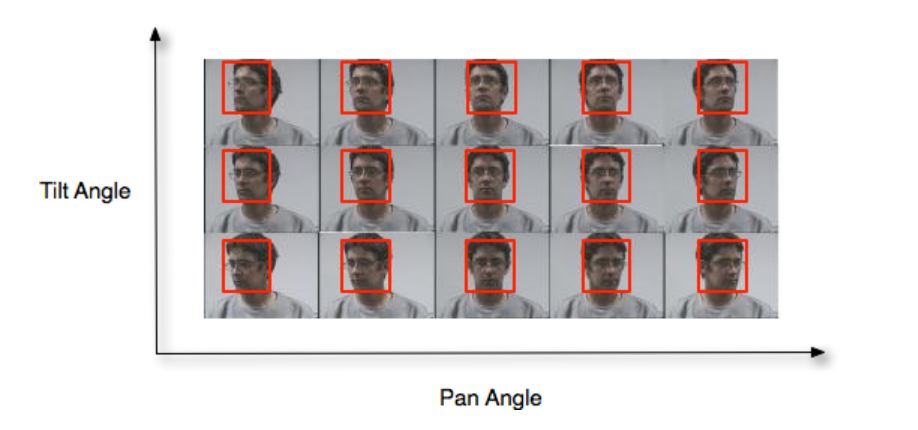
\includegraphics[scale=1]{figures/tiltpan.png}
	\caption{Muestra de 15 fotografías del sujeto 12 \cite{Gourier_Hall_Crowley}}
	\label{fig:img0}
\end{figure}

\begin{figure}[H]
	\centering
	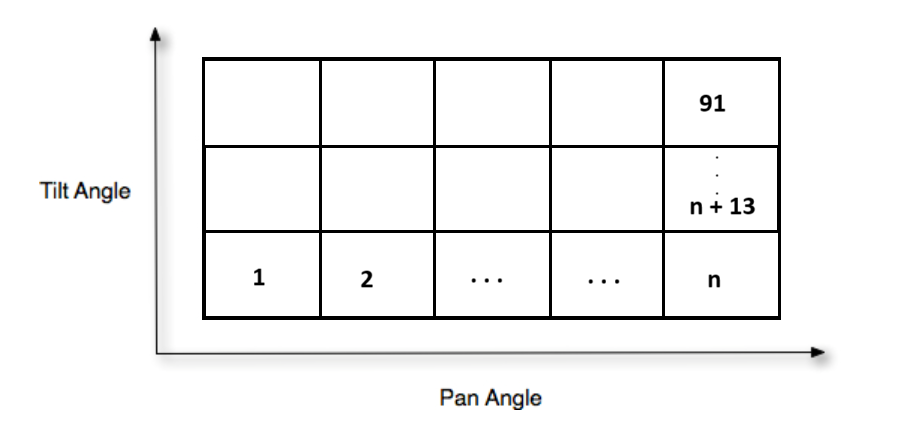
\includegraphics[scale=1]{figures/faceorder.png}
	\caption{Orden de guardado para cada serie de fotografías}
	\label{fig:img1}
\end{figure}

Además de este orden, todas las series de fotografías iniciaban con la imagen de la cabeza completamente hacia arriba y finalizaban con la posición completamente abajo, de frente para ambas. Dado que se tenían 15 sujetos de prueba, se procedió a guardar los archivos JPG de 11 (2046 imágenes) sujetos en un directorio de entrenamiento y los 4 (744 imágenes) restantes en el de pruebas. Al tener en cuenta el orden de los archivos y la cantidad en cada directorio se procedió a realizar las etiquetas por medio de un documento \textit{Excel}con formato \textit{.xlsx}. En dicho documento se creó una hoja para cada grupo de etiquetas, esto quiere decir, una hoja para etiquetas de entrenamiento y otra para etiquetas de prueba. Por lo que, en cada hoja se puede encontrar una columna con las etiquetas en el orden establecido en la Figura 2.

\subsection{Etiquetas para clasificación}

Para la primera experimentación se consideró clasificar las imágenes en 9 clases diferentes, de tal manera que la orientación de la cabeza respecto de la cámara funcionara de manera similar a una palanca de mandos analógica. A continuación se presenta una visualización de dicha clasificación:

\begin{figure}[H]
	\centering
	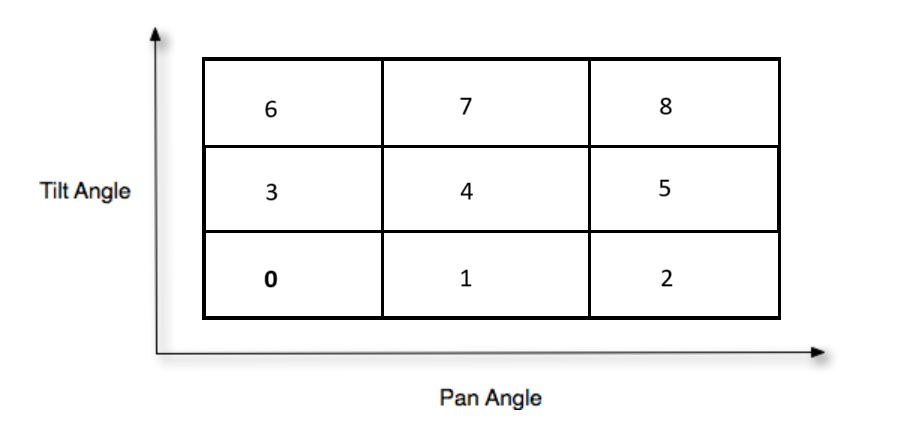
\includegraphics[scale=1]{figures/clasi0.png}
	\caption{Clasificación de imágenes en 9 etiquetas}
	\label{fig:img2}
\end{figure}

Utilizando esta cantidad de clases, se realizaron dos formas de etiquetado en las imágenes, en las cuales solo varía la cantidad de fotografías que fueron etiquetadas dentro de una clase u otra. En las siguientes figuras se podrá observar que la dimensión de cada celda está representada con (n $\times$ m), dónde n corresponde a la cantidad de ángulos panorámicos que abarca y m la cantidad de ángulos de inclinación (según las muestras tomadas del ICPR). Además, la posición de las celdas en las gráficas si corresponde a la numeración de la Figura 2.


\begin{figure}[H]
	\centering
	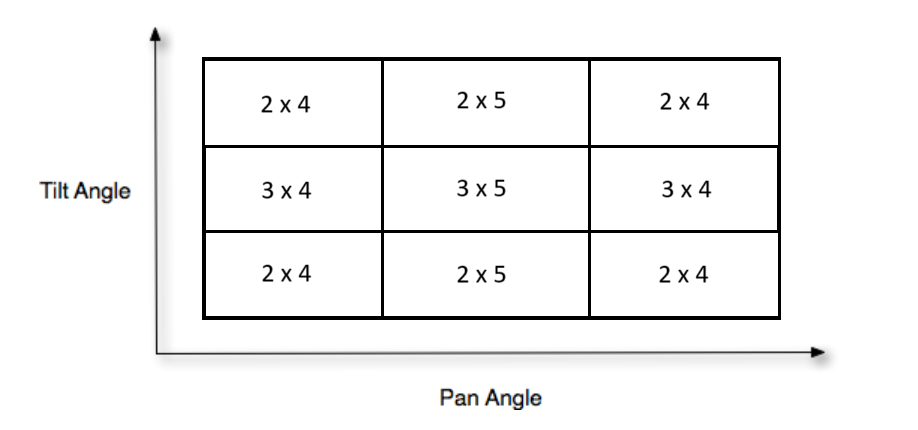
\includegraphics[scale=1]{figures/clasi01.png}
	\caption{Primera distribución de etiquetas}
	\label{fig:img3}
\end{figure}

\begin{figure}[H]
	\centering
	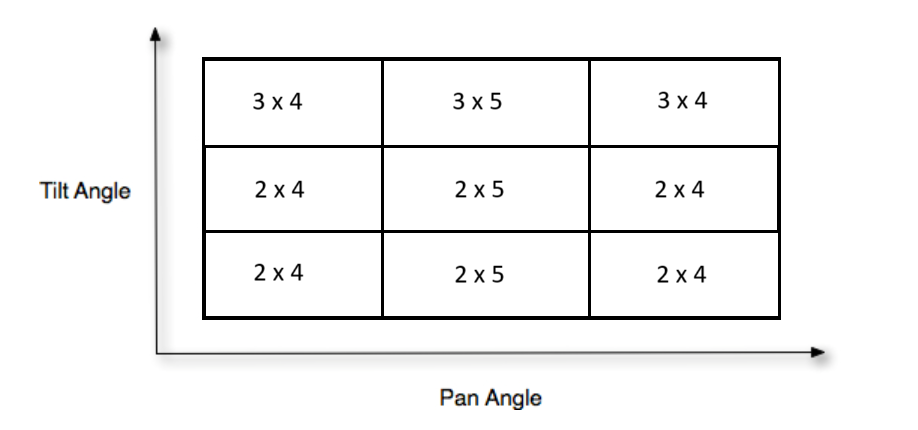
\includegraphics[scale=1]{figures/clasi02.png}
	\caption{Segunda distribución de etiquetas}
	\label{fig:img4}
\end{figure}

Luego de pruebas realizadas con resultados no satisfactorios en la sección de algoritmos para visión por computadora, la siguiente experimentación consistió en reducir la cantidad de clases a 6. En este caso para realizar un movimiento hacia atrás, se requiere un giro completo, en vez del sistema de joystick propuesto anteriormente. La división de clases se muestra a continuación:

\begin{figure}[H]
	\centering
	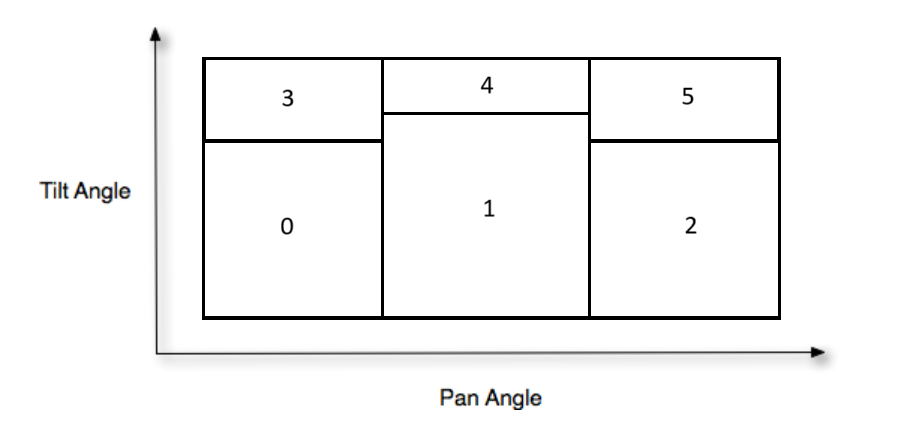
\includegraphics[scale=1]{figures/clasi1.png}
	\caption{Clasificación de imágenes en 6 etiquetas}
	\label{fig:img5}
\end{figure}

\begin{figure}[H]
	\centering
	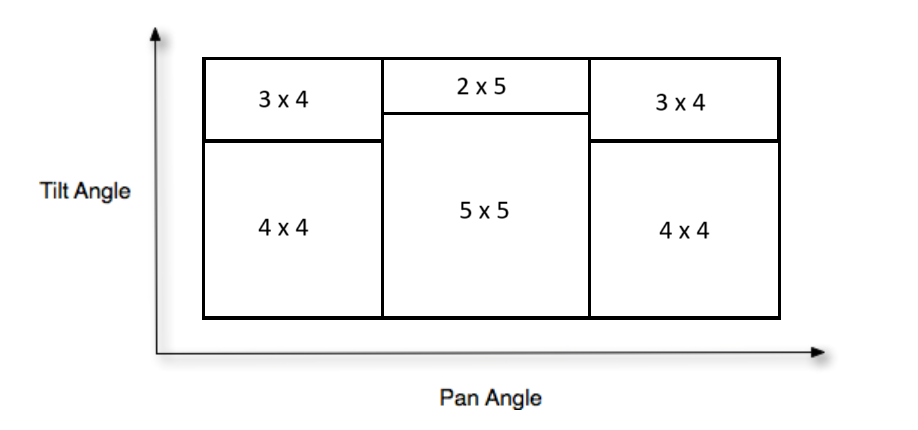
\includegraphics[scale=1]{figures/clasi2.png}
	\caption{Tercera distribución de etiquetas}
	\label{fig:img6}
\end{figure}

\begin{figure}[H]
	\centering
	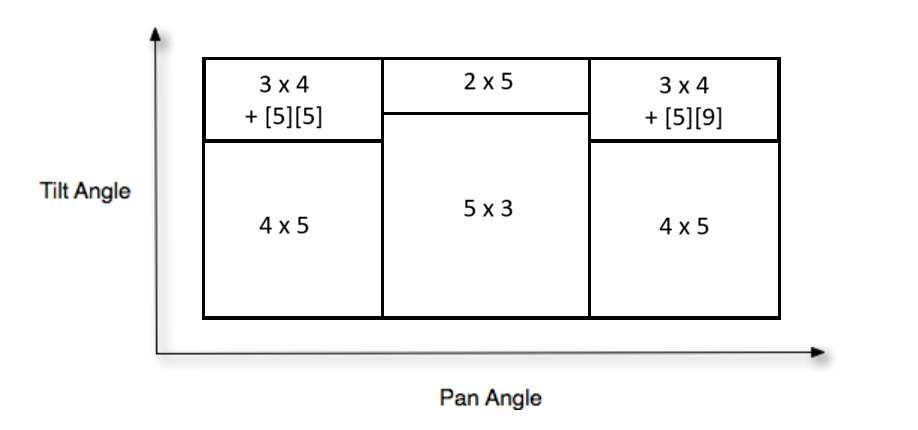
\includegraphics[scale=1]{figures/clasi3.png}
	\caption{Cuarta distribución de etiquetas (Las posiciones se cuentan desde la esquina inferior izquierda)}
	\label{fig:img7}
\end{figure}


\subsection{Fotografías personales}
Dado que los resultados con los modelos de de reconocimiento de orientación no fueron los esperados en ningún caso, se procedió a realizar dos series de fotografías personales con la cámara integrada. Cada serie consta de 9 fotografías con posiciones que simulan las 9 clases inicialmente definidas a una distancia de 45 cm aproximadamente. Una de las series fue tomada en un salón de laboratorio del Departamento de Ingeniería Electrónica, Mecatrónica y Biomédica de la Universidad del Valle de Guatemala y la otra fue realizada en un espacio de trabajo en la casa de Gerardo Andres Fuentes Bámaca (autor). Luego, las fotografías fueron renombradas de tal manera que se pudiera conocer su orden y posición en la lista de imágenes del grupo de entrenamiento. De esta manera, fueron agregadas las etiquetas correspondientes en el documento de etiquetas con extensión \textit{.xlsx}, tanto para los casos de 9 y 6 clases.
\section{ColorFET}
\chapter{Algoritmos para visión por computadora}
\section{Preprocesado de imágenes}


Inicialmente se diseñó un código para extraer fotografías desde un directorio, etiquetas desde un documento con extensión \textit{.xlsx} y luego transformarlos en matrices de datos que para poder ser utilizados en los proceso de \textit{Machine Learning}. Para la realización de este código, se utilizaron las siguientes librerías: \textit{OS}, \textit{CV2 (OpenCV)}, \textit{Numpy} y \textit{Pandas}. Además de esto el proceso para la realización del código fue el siguiente: 

\subsection{Transformación de fotografías}
En este caso, se utilizó la librería \textit{OS} para crear una lista con nombres en formato cadena de los archivos en un directorio dado. Luego, utilizando la librería \textit{Numpy}, se creó una matriz de ceros para guardar todas las fotografías convertidas en formato de matriz. Para realizar la conversión, previamente se realizó una prueba para obtener las dimensiones mínimas con las que puede trabajar la cámara integrada con la librería \textit{CV2}, cuyo tamaño es 320 $\times$ 180 píxeles. Después, dentro de un bucle \textit{for} se utilizó la librería \textit{CV2} obtener la matriz de pixeles de cada fotografía, ajustar el tamaño a las dimensiones encontradas y luego transformar el canal de color por defecto BGR \textit{(Blue, Green, Red)} a RGB \textit{(Red, Green, Blue)}. 

\subsection{Transformación de etiquetas}

Para transformar las etiquetas en matrices de datos, únicamente se requirió la librería \textit{Pandas}, ya que nos permite utilizar una función específica para leer documentos con formato \textit{.xlsx}, así como acceder a las hojas internas del documento. Al guardar el resultado de esta función el siguiente paso es convertirlo a un formato de matriz con funciones de \textit{Numpy}. 

\subsection{Exportación de datos finales}

La librería \textit{Numpy} cuenta con una función para exportar matrices de datos de manera individual (una variable a la vez), o bien agruparlas en un solo archivo. En este caso, se guardaron las matrices de fotografías en un solo archivo, dado que estas solo cambiarán si se agregan más fotografías. Por otro lado, las matrices de etiquetas fueron exportadas de manera individual dado que se cuenta con diferentes grupos.

\section{Entrenamiento de modelos de \textit{machine learning}}
Para las primeras pruebas se utilizó el framework \textit{TensorFlow y Keras} para poder realizar los diferentes modelos de \textit{Machine Learning} para reconocimiento de orientación de cabeza, utilizando las matrices de datos obtenidas a partir de la base de datos de ICPR. Para este código se utilizaron las librerías \textit{TensorFlow}, \textit{Matplotlib}, \textit{Numpy} y \textit{Seaborn}. El código fue realizado de la siguiente manera:

\subsection{Extracción de datos previamente procesados}
Luego de exportar los archivos transformados de la base de datos, se generan archivos con extensión \textit{.npy} para los archivos de una variable y \textit{.npz} para los de múltliple variables. Dichos archivos pueden ser importados utilizando también funciones de la librería \textit{Numpy}, para guardarlos en variables utilizables dentro del código, optimizando así el tiempo de transformación de datos.

\subsection{Modelo de reconocimiento de orientación de cabeza}
El primer pasó fue normalizar los valores de las matrices, dado que son imágenes RGB, cada píxel de estas está representado por 3 valores que varían entre 0 y 255, y se necesitan valores entre 0 y 1, por lo que únicamente se tuvo que dividir tanto la variable con datos de entrenamiento y de prueba entre el valor 255. 
\section{Ajuste de modelos preentreanados}
\section{Pruebas en tiempo real}


\chapter{Traducción algoritmo a comandos}

%Esta etapa contempla la iteración de pruebas para conseguir un algoritmo que funcione de manera efectiva al reconocer los gestos y movimientos de la cabeza del usuario. Luego de obtener un reconocimiento efectivo, se generarán diferentes ítems, clases o divisiones para cada tipo de gestos. Al tener definida la lista de tipos, se procede a utilizarlos para generar comandos genéricos para poder utilizar los agentes robóticos móviles simulados y físicos.

\chapter{Simulaciones}

%El algoritmo anterior será utilizado para realizar simulaciones de movimiento/envío de comandos en diferentes escenarios. Para poder ejecutar dichas pruebas, será necesario también realizar un análisis de los diferentes simuladores disponibles, los cuales sean compatibles con los algoritmos determinados anteriormente. Se realizará un registro de datos de las iteraciones realizadas para analizarlas de manera estadísticas y determinar el comportamiento de cada algoritmo según el escenario propuesto. De esta manera, se podrá partir con datos o comandos iniciales para las pruebas físicas. Los escenarios a probar constan del entorno físico alrededor del robot, así como los diferentes gestos a utilizar. 

\chapter{Pruebas físicas}

%Al obtener los parámetros iniciales determinados en las simulaciones, se empezará la migración de estos, junto con los algoritmos, hacia los robots a utilizar. En primer lugar se realizará una comparación entre los resultados obtenidos de manera física contra las simulaciones. Las pruebas físicas se realizarán en diferentes condiciones, como el de luminosidad, o el de contenido visual con diferentes niveles de ruido para tener un rango de operación más grande. También, las pruebas físicas tendrán un análisis cada algoritmo con diferentes variaciones en parámetros iniciales o en el algoritmo por sí mismo. De esta manera se podría verificar el alcance del sistema en conjunto, del robot, el sensor y el algoritmo seleccionado. También, se realizarán pruebas con diferentes sujetos de control, es decir diferentes personas realizando los gestos para controlar el movimiento del robot. Al realizar las pruebas, también se guardaran los datos obtenidos a partir de los sensores de tal manera que se puedan clasificar dependiendo del gesto utilizado. 

\fi

% CONCLUSIONES
% ------------------------------------------------------------------------------
\ifdefined\CAPconclusiones
	\newpage
	\chapter{Conclusiones}
	\ifdefined\parpordefecto
		\defaultparformat{k-conclusiones}
	\else
		\input{k-conclusiones}
	\fi
\fi

% RECOMENDACIONES
% ------------------------------------------------------------------------------
\ifdefined\CAPrecomendaciones
	\newpage
	\chapter{Recomendaciones}
	\ifdefined\parpordefecto
		\defaultparformat{l-recomendaciones}
	\else
		\input{l-recomendaciones}
	\fi
\fi

% BIBLIOGRAFÍA
% ------------------------------------------------------------------------------
\ifdefined\CAPbibliografia
	\newpage
    \cleardoublepage\phantomsection
	\chapter{\bibname}
    \printbibliography[heading=none]
\fi

% ANEXOS
% ------------------------------------------------------------------------------
\ifdefined\CAPanexos
	\newpage
	\chapter{Anexos}
	\ifdefined\parpordefecto
		\defaultparformat{n-anexos}
	\else
		\section{hola mundo}
	\fi
\fi

% GLOSARIO
% ------------------------------------------------------------------------------
\ifdefined\CAPglosario
	\newpage
	\printglossary
\fi

\end{document}